\documentclass[11pt]{article}
\title{Comparison of Convolutional Neural Networks for Remote Sensing}
\date{2018-05-09}
\author{James Hurt}
\usepackage[margin=1.0in]{geometry}
\usepackage{graphicx}
\usepackage{subcaption}
\usepackage{cleveref}
\usepackage{indentfirst}
\begin{document}
	\pagenumbering{arabic}
	
	%%%%%%%%%%%%%%%%
	% Title 
	%%%%%%%%%%%%%%%%
	\begin{flushright}
		James Hurt\break
		CS 8780\break
		9 May 2018
	\end{flushright}
	\begin{center}
		\huge{Comparison of Convolutional Neural Networks for Remote Sensing}
	\end{center}
	
	%%%%%%%%%%%%%%%%%%%%%%%
	% Technical Description
	%%%%%%%%%%%%%%%%%%%%%%%

	\begin{figure}[b!]
			\centering
			\begin{subfigure}[b]{0.3\linewidth}
				\centering
				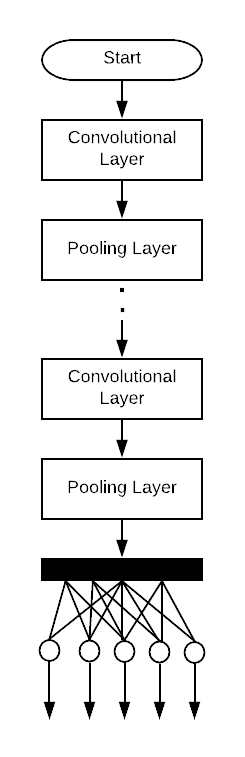
\includegraphics[scale=0.38]{img/custom_arc.png}
				\caption{Custom Shallow CNN}
				\label{fig:shallow_cnn}
			\end{subfigure}
			\begin{subfigure}[b]{0.3\linewidth}
				\centering
				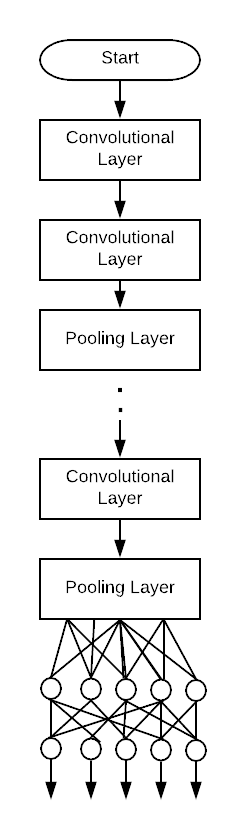
\includegraphics[scale=0.34]{img/vgg.png}
				\caption{VGG19}
			    \label{fig:deep_cnn}
			\end{subfigure}
			\begin{subfigure}[b]{0.3\linewidth}
				\centering
				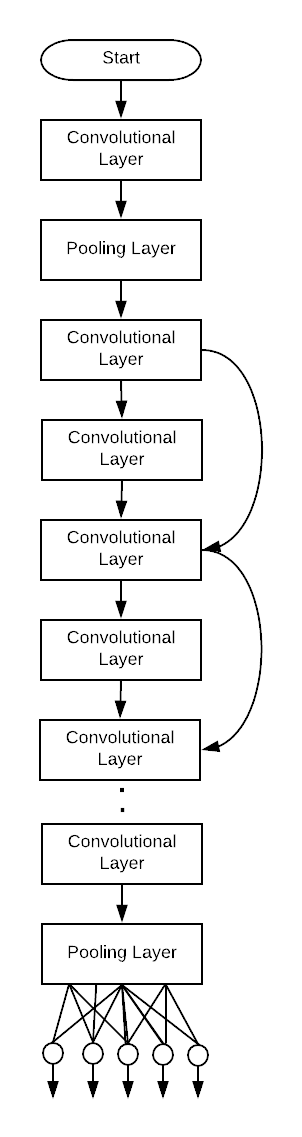
\includegraphics[scale=0.25]{img/res50.png}
				\caption{ResNet-50}
				\label{fig:deep_rnn}
			\end{subfigure}
			\caption{Architectures of the Compared CNN}
			\label{fig:architecture}
		\end{figure}

	\section{Technical Description}
	
		Remote Sensing is a lucrative application for computational intelligence, with much of the recent research being in Convolutional Neural Networks. Within this discussion of neural networks for remote sensing, Deep Convolutional Neural Networks (DCNN) are the most popular. The popularity of convolutional neural networks can be attributed to the ability of a convolutional network to learn the features of the image, thus eliminating one of the greatest challenges in all of machine learning: feature selection and extraction. While CNN have proven very useful, one of the issues with DCNN is the high training time, even with GPU acceleration. In this project, I attempt to compare a shallow convolutional network with one of the first deep convolutional networks. I then take my comparison one step farther, by looking at the relative cost and benefit of residual neural networks. 
		
		\subsection{Shallow Convolutional Neural Network}
		
The shallow convolutional neural network used in this project combines many techniques of fully connected networks previously used for pattern recognition. The architecture of the network can be see in \Cref{fig:shallow_cnn}.
		
The architecture of the network has a total of 12 layers. The first 10 layers are alternating 2D Convolutional layers layers with a 3x3 kernel size and 2D Max Pooling layers with a 2x2 Pooling Window. After these 10 layers, feature extraction is finished, and a flattening layer is introduced to put the data into a single vector for the final fully connected softmax layer. 
		
		
		\subsection{Deep Convolutional Neural Network}
		
The Deep Convolutional Neural Network used for comparison in this project is VGG 19 \cite{vgg}. The VGG 19 network, as the name suggests, has 19 total layers. This count, however, does not include the pooling layers. The basic architecture can been seen in \Cref{fig:deep_cnn}. There are 16 convolutional layers and 4 pooling layers. The final pooling layer is then connected to 3 fully connected layers, the last of which is a softmax layer for classification. 
		\subsection{Deep Residual Convolutional Neural Network}
	
	\section{Algorithm Design}
	
	\section{Experiment Results}
	
	\section{Analysis}
	
	\section{Code}
	
	

	\newpage
	\bibliography{bibliography} 
	\bibliographystyle{ieeetr}




\end{document}